\documentclass[12pt,letterpaper,notitlepage]{report}
\usepackage{setspace}
\usepackage{natbib}
\usepackage{epstopdf}
\usepackage{graphicx}
\usepackage[font={small,it},width=0.8\textwidth]{caption}

\setlength{\parskip}{2em}
\setlength{\intextsep}{2.5em}

\begin{document}

\title{Experimental Demonstrations of Superconducting Charge Qubits}
\author{John Meade}
\date{April 6, 2015}

\maketitle

%%%%%%%%%%%%%%%%%%%%%%%%%%%%%%%%%%%%%%%%%%%%%%%%%%
% Abstract
\begin{abstract}
\doublespacing
\noindent
Superconducting circuits provide interesting ways to achieve qubit systems, along with many engineering challanges and hence new physics. One such type of system is the charge qubit, which has passed several milestones over the past few years. This paper will make use of several papers to review these recent successes, namely the demonstration of a single coherent qubit \cite{singleCooperPair} and subsequent demonstrations of entangled two-qubit systems \cite{twoPulseGates}\cite{onePulseGateNature}\cite{onePulseGatePhysica}.
\end{abstract}

%%%%%%%%%%%%%%%%%%%%%%%%%%%%%%%%%%%%%%%%%%%%%%%%%%
% Main
\pagebreak
\doublespacing

%
%   General Info / Background
%

\section*{General Info}

The Cooper pair box (CPB), shown in Fig. 1, is the starting point for charge-based superconducting qubits. In this device, there is a thin insulating layer between the two chunks of superconducting metal (grey boxes), acting as an electron tunneling junction. Due to the low temperature of the system, electrons condense into Cooper pairs due to an electron-phonon interaction, leading to the superconductivity. Small circuits like this, under superconducting conditions, will exhibit Josephson effects. That is, there will be a current flowing across the insulator due to tunneling.

First, an outline of how a CPBs can be turned into a qubit will be presented. The general idea is to base the state of the qubit on the number of excess Cooper pairs are on the \"island\" of the CPB. Certain fabrication constraints on the cicuits must be imposed to obtain a usable coherent qubit, such as sub-femto Farad capacitors and specific relationships between energies of the system (Josephson, coupling, and charging energies). Under correct conditions, only Cooper pairs will tunnel, and the system Hamiltonian is

$H=4E_c(n-n_g)^2-E_Jcos\Theta$

Where $E_C$ is the charging energy, $n$ is the number operator of excess Cooper pairs, $n_g=C_gV_g/2e$ is the number operator control parameter due to the gate voltage, $E_J$ is the Josephson coupling energy, and $\Theta$ is the phase difference across the junction.

edit this shit... refer to \cite{reviewPaper} for a detailed introduction to superconducting qubits

%
%   Fabrication
%

\section*{Fabrication}

% could throw some pictures in here
[images]

Typical fabrication techniques exist for these superconducting devices, and a possible procedure for making and operating them is as follows \cite{onePulseGatePhysica}. The circuit metal used is aluminum, which is evaporated onto a substrate. A mask for shadow evaporation is prepared using electron-beam lithography and dry etching, which allows overlapping aluminum structures to be fabricated. Exposing aluminum to oxygen at set pressure and time causes a layer of oxidation to build up on the surface, which provides a convenient tunnel junction. Different times and pressures are ued to acheive different junction parameters for Josephson junctions and probe junctions. The final circuit is operated in a dilution fridge with a mixing chamber temperature of about 40mK.

%
%   One-Qubit Experiments
%

\section*{One-Qubit Experiments}

One idea for one-qubit experiments is to fabricate a SQUID and control it with a pulse gate (effectively a capacitor). The island on this device holds some ground-state number of Cooper pairs. We identify this as the $|0\rangle$ state, and define $|1\rangle$ to be the ground state plus one extra Cooper pair. We can then control the evolution of this qubit coherently with a voltage pulse.

\begin{figure}[ht]
    \centering
    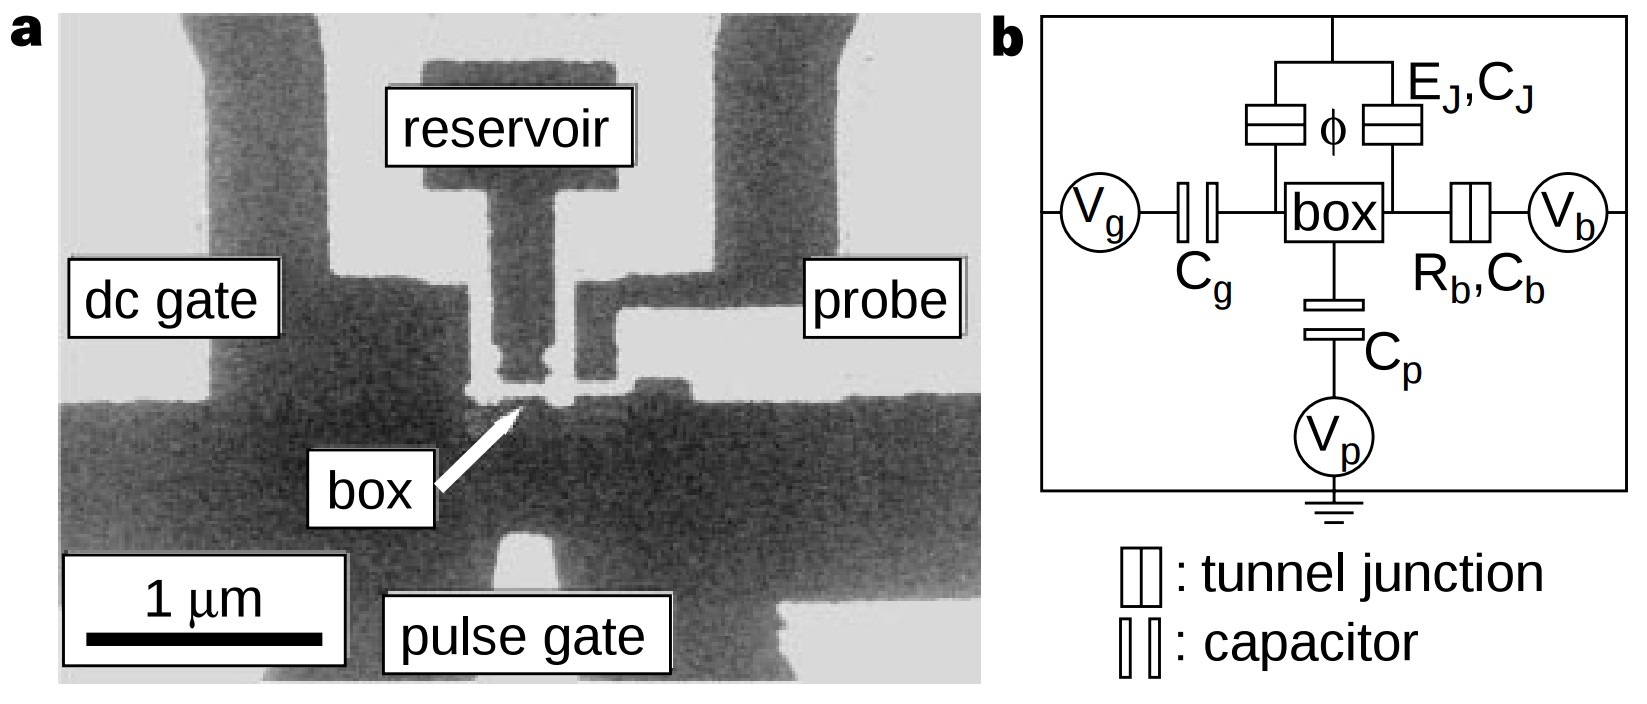
\includegraphics[width=\textwidth]{img/nakamura-single-cpb.jpg}
    \caption{SEM image of a superconducting device for a single charge qubit (Nakamura, Pashkin, Tsai, 1999) \cite{singleCPB}}
\end{figure}

Figure 1 shows an implementation of a single-qubit device. The DC gate can be controlled to tune the state of the qubit by creating an induced charge. This can be set to a value that makes it very unlikely for any charge oscillations (due to Josephson coupling) to occur, and thus by waiting an appropriate amount of time the system can be assumed to have decayed into a pure ground state.

Due to Josephson coupling, the system will exhibit an oscillating behaviour when the total induced charge reaches certain values. The idea here is to initialize the qubit with the gate voltage, and then apply a sharp pulse with the pulse gate. This will non-adiabatically drive the system into resonance between ground and excited state for the pulse duration.

The state measurements are done with the probes. These probes measure current, which is caused by quasiparticles tunneling through the probe junction from the excited qubit state. The probes are connected throughout the qubit evolution (the length of the pulse), so they must have a fairly high tunnel resistance to keep decoherence down.

A single voltage pulse may not produce a measurable signal \cite{singleCPB}, so a technique using arrays of pulses is often employed. This involves performing many pulses separated by a time $T_r$, such that $T_r$ is longer than the qubit relaxation time. Through this method, you find that the current peaks measured do not depend on $T_r$, and so only depend on the pulse length.

\begin{figure}[ht]
    \centering
    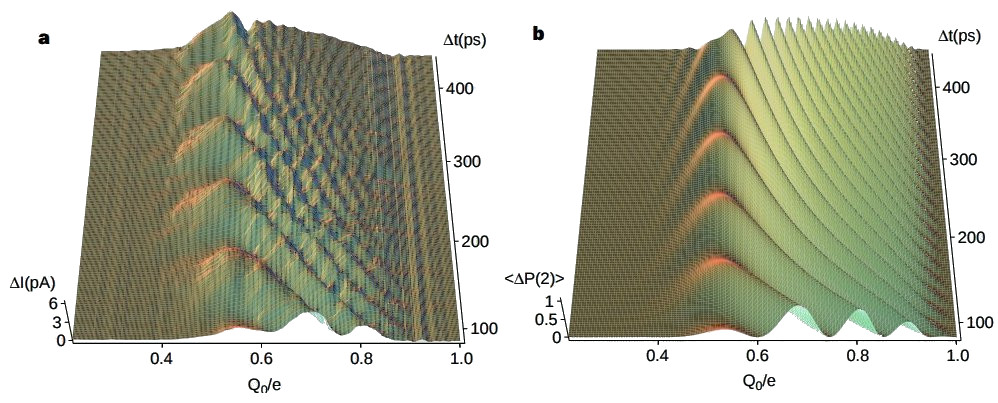
\includegraphics[width=\textwidth]{img/nakamura-pulse-response.jpg}
    \caption{Effect of applying pulses as a function of DC induced charge $Q_0$ and pulse length $\Delta t$ (Nakamura, Pashkin, Tsai, 1999) \cite{singleCPB}. Colours inverted for printing.}
\end{figure}

Figure 2a shows the oscillating current response caused by the pulse, for various values of the induced charge from the gate voltage. Figure 2b was generate by numerically solving a time dependent Schr{\"o}dinger equation. The agreement between these figures shows that the theory accurately predicts the oscillations between qubit states. Further discussion of these coherent oscillations can be found in \cite{singleCPB}.

%
%   Two-Qubit Experiments
%

\section*{Two-Qubit Experiments}

Since the demonstration of single coherent qubits, groups began expirimenting with two-qubit systems. The model we will follow for this section is a circuit consisting of a CPB capacitively coupled to a SQUID-controlled box. This coupling should act as a channel in which the qubits can entangle with each other.

\begin{figure}[ht]
    \centering
    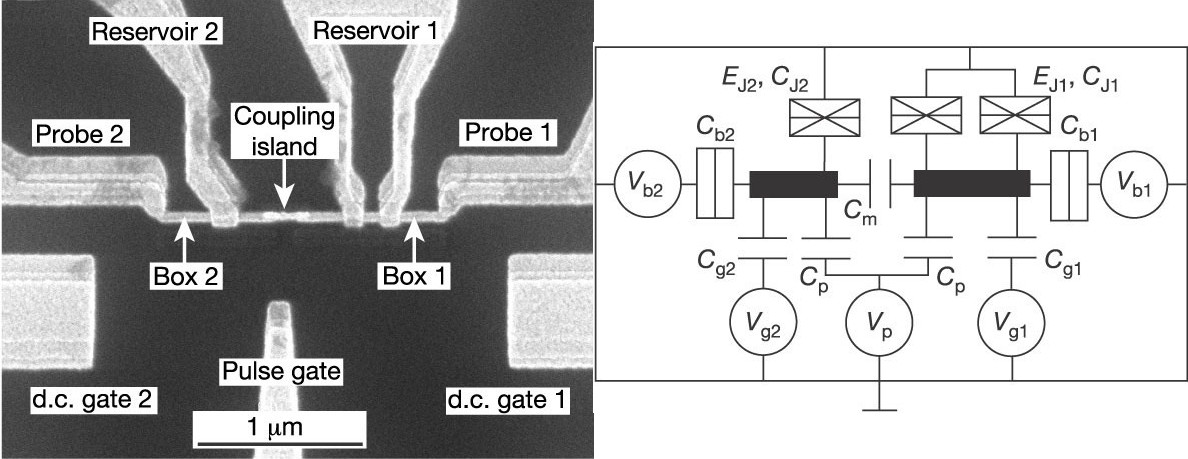
\includegraphics[width=\textwidth]{img/two-qubit-circuit.jpg}
    \caption{SEM of two-qubit device with equivalent circuit diagram (Nakamura, Pashkin, Tsai, 2003) \cite{onePulseGateNature}}
\end{figure}

Figure 3 shows a circuit for such an experiment. Note the pulse gate, which is common to, and approximately equally coupled to, both qubits. This circuit is designed such that parameters of the circuit can be estimated (charging energies, Josephson energies, etc).

\begin{figure}[ht]
    \centering
    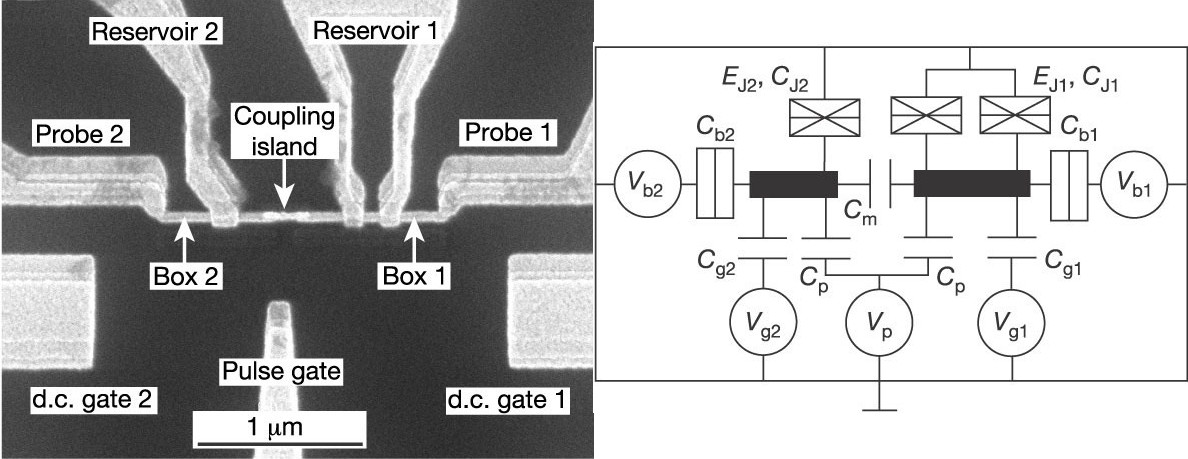
\includegraphics[width=\textwidth]{img/two-qubit-circuit.jpg}
    \caption{SEM of two-qubit device with equivalent circuit diagram (Nakamura, Pashkin, Tsai, 2003) \cite{onePulseGateNature}}
\end{figure}

%%%%%%%%%%%%%%%%%%%%%%%%%%%%%%%%%%%%%%%%%%%%%%%%%%
% Bib
\bibliographystyle{plain}
\bibliography{charge-qubits}

\end{document}
